\documentclass{article}
\usepackage{arxiv}

\input{math_commands.tex}

\usepackage{microtype}
\usepackage{graphicx}
\usepackage{booktabs}
\usepackage{tabularx}
\usepackage{hyperref}
\usepackage{caption}
\usepackage{subfigure}
\usepackage{float}
\usepackage{enumitem}
\usepackage{placeins}
\usepackage{xurl}
\Urlmuskip=0mu plus 1mu
\usepackage[numbers,sort]{natbib}

% Match the original KernelBench paper page layout.
\setlength{\textwidth}{6.5in}
\setlength{\textheight}{9in}
\setlength{\oddsidemargin}{0in}
\setlength{\evensidemargin}{0in}
\setlength{\topmargin}{-0.5in}

% Auto-generated from results.csv
\newcommand{\TotalEvals}{738}
\newcommand{\TotalModels}{9}
\newcommand{\TotalGPUs}{2}
\newcommand{\TotalProblems}{41}
\newcommand{\TotalPassed}{313}
\newcommand{\TotalCompiled}{439}
\newcommand{\TotalCorrect}{313}
\newcommand{\TotalBeats}{146}
\newcommand{\TotalTokens}{35582950}
\newcommand{\TotalCost}{114.20}
\newcommand{\AvgSpeedup}{1.522}
\newcommand{\SpeedupCount}{313}
\newcommand{\OverallPassRate}{42.4}
\newcommand{\OverallBeatRate}{19.8}
\newcommand{\PassRateLOne}{57.8}
\newcommand{\BeatRateLOne}{19.3}
\newcommand{\PassRateLTwo}{43.0}
\newcommand{\BeatRateLTwo}{31.5}
\newcommand{\PassRateLThree}{44.4}
\newcommand{\BeatRateLThree}{5.6}
\newcommand{\PassRateLFour}{11.8}
\newcommand{\BeatRateLFour}{4.2}


\title{KernelBench v3: Rebuilding a GPU Kernel Benchmark from First Principles}
% Author block using authblk to match the original KernelBench paper layout.
\usepackage{authblk}

\author[1]{Elliot Arledge}


\begin{document}

\maketitle

\begin{abstract}
Efficient GPU kernels are essential for modern ML systems, but kernel engineering remains expensive and specialized. KernelBench v3 is a benchmark for evaluating whether large language models can produce optimized CUDA kernels that are both correct and faster than established PyTorch baselines. We rebuild KernelBench with a smaller, higher quality task set focused on modern architectures, and we report results across \TotalModels{} models, two GPUs, and \TotalProblems{} problems. Across \TotalEvals{} evaluations, \OverallPassRate\% pass correctness checks and \OverallBeatRate\% beat the baseline. The most capable models can beat the baseline on many Level 1 and 2 tasks, but performance collapses on Level 4 problems that use novel architectures or already-optimized Triton baselines. These results highlight the gap between code generation and production-grade kernel engineering.
\end{abstract}

\section{Introduction}
Kernel engineering is a bottleneck for deploying efficient ML systems. While modern compilers and libraries provide optimized kernels, tailoring kernels to new architectures or fused operators often requires expert attention. Recent work introduced KernelBench to test whether LLMs can automate this process by producing faster CUDA kernels from PyTorch reference code~\cite{kernelbench}. The benchmark sparked interest, but subsequent analyses showed that benchmark design and evaluation details strongly influence results~\cite{metr2025}.

KernelBench v3 is a rebuild focused on modern inference kernels, stronger baselines, and transparent cost accounting. The benchmark reduces the problem set to 41 tasks that are representative of current workloads, prioritizes Hopper and Blackwell GPUs, and tracks per-run tokens and cost. The goal is not to maximize speedups with fragile tricks, but to measure whether models can produce kernels that compile, are numerically correct, and outperform real baselines.

This paper makes three contributions:
\begin{itemize}[leftmargin=1.2em]
    \item A curated benchmark of 41 modern kernel tasks across four difficulty levels.
    \item An evaluation pipeline that reports compilation, correctness, and baseline-beating rates, with full per-run cost accounting.
    \item A results summary across \TotalModels{} models on H100 and B200 GPUs, highlighting where current models still fail.
\end{itemize}


\section{Background and Motivation}
KernelBench v0.1 and the original KernelBench paper established a useful framing: models are given a PyTorch reference implementation and must produce a faster CUDA kernel~\cite{kernelbench,stanford-kernelbenchv01}. Subsequent investigations revealed several reward-hacking patterns, including calling high-level libraries instead of writing kernels, manipulating timing, or exploiting numerically trivial tasks~\cite{metr2025}. These findings motivated a ground-up redesign rather than incremental fixes.

KernelBench v3 is designed with two principles. First, tasks should reflect modern kernel engineering needs, including fused matmul chains, attention blocks, and emerging linear-attention variants. Second, baselines should be meaningful: for some Level 4 tasks, the baseline is already an optimized Triton implementation, so beating the baseline requires genuinely competitive kernel engineering.

This redesign also emphasizes cost realism. Running large model sweeps across many problems and hardware targets can become prohibitively expensive. KernelBench v3 focuses on two widely deployed data center GPUs and a smaller, curated task set while preserving the evaluation challenge.


\section{Benchmark Design}
KernelBench v3 contains 41 tasks across four levels (Table~\ref{tab:levels}). Each task provides a PyTorch reference model and an input generator. The model under evaluation must produce a CUDA implementation that matches the reference output and improves runtime. Level 1 contains basic kernels such as matmul, softmax, and normalization. Level 2 contains fused multi-op patterns such as matmul-plus-activation-plus-norm chains. Level 3 covers single attention blocks and a transformer block. Level 4 focuses on modern inference kernels, including DeepSeek-style MLA and MoE patterns~\cite{deepseek-v3}, GQA~\cite{gqa}, FP8 and INT4 matmuls~\cite{fp8-formats,int4-quant}, and linear-attention variants such as Gated DeltaNet and Kimi Delta Attention~\cite{gated-deltanet,kimi-linear}.

Some Level 4 baselines are already optimized Triton implementations~\cite{triton}. For example, the Gated DeltaNet and Kimi Delta Attention tasks use optimized kernels rather than naive PyTorch baselines, which sets a high bar for LLM-generated code. As a result, Level 4 performance reflects whether models can compete with production-quality kernels rather than only outperform naive baselines.

\begin{table}[t]
\centering
\caption{KernelBench v3 levels and turn limits.}
\label{tab:levels}
\begin{tabular}{cccc}
\toprule
Level & Tasks & Turns & Description \\
\midrule
L1 & 15 & 10 & Simple ops: matmul, softmax, conv, norms \\
L2 & 15 & 12 & Fused ops: matmul and activation chains \\
L3 & 3 & 15 & Single blocks: attention and transformer block \\
L4 & 8 & 15 & Novel layers: MLA, MoE, GQA, FP8, INT4, DeltaNet \\
\bottomrule
\end{tabular}
\end{table}

KernelBench v3 evaluates on two target GPUs: H100 (Hopper) and B200 (Blackwell)~\cite{nvidia-h100,nvidia-b200}. The benchmark runs in a Modal sandbox with CUDA 13.1~\cite{modal-docs,cuda-13-1}, providing a consistent environment for compilation and benchmarking.


\section{Evaluation Methodology}
Each evaluation is a multi-turn agent loop. The model receives a PyTorch reference implementation, GPU target, and constraints, then iteratively proposes CUDA code. We cap the number of turns per problem by level (Table~\ref{tab:levels}) to control cost.

\paragraph{Compilation.} A submission is marked \emph{compiled} if the generated code defines the required model class and executes without errors in the Modal sandbox~\cite{modal-docs}.

\paragraph{Correctness.} A compiled kernel is considered correct if its output matches the reference model within a tolerance. The evaluation script computes the maximum absolute error and compares it to \texttt{atol + rtol * max(|ref|)} with \texttt{atol=0.05} and \texttt{rtol=0.02}.

\paragraph{Performance.} We time the reference model and the generated kernel over 10 iterations with CUDA synchronization, after a short warmup. Speedup is defined as the reference runtime divided by the candidate runtime. A kernel \emph{beats the baseline} when its speedup exceeds 1.0.

\paragraph{Metrics.} We report compilation rate, correctness rate, and baseline-beating rate. For each run, we also log tokens and estimated API cost, enabling cost-adjusted analysis.


\section{Results}
We report results over \TotalEvals{} evaluations covering \TotalModels{} models, two GPUs, and \TotalProblems{} problems. Overall, \OverallPassRate\% of runs pass correctness and \OverallBeatRate\% beat the baseline. The average speedup among correct kernels is \AvgSpeedup{}x over \SpeedupCount{} successful runs.

\begin{figure}[t]
\centering
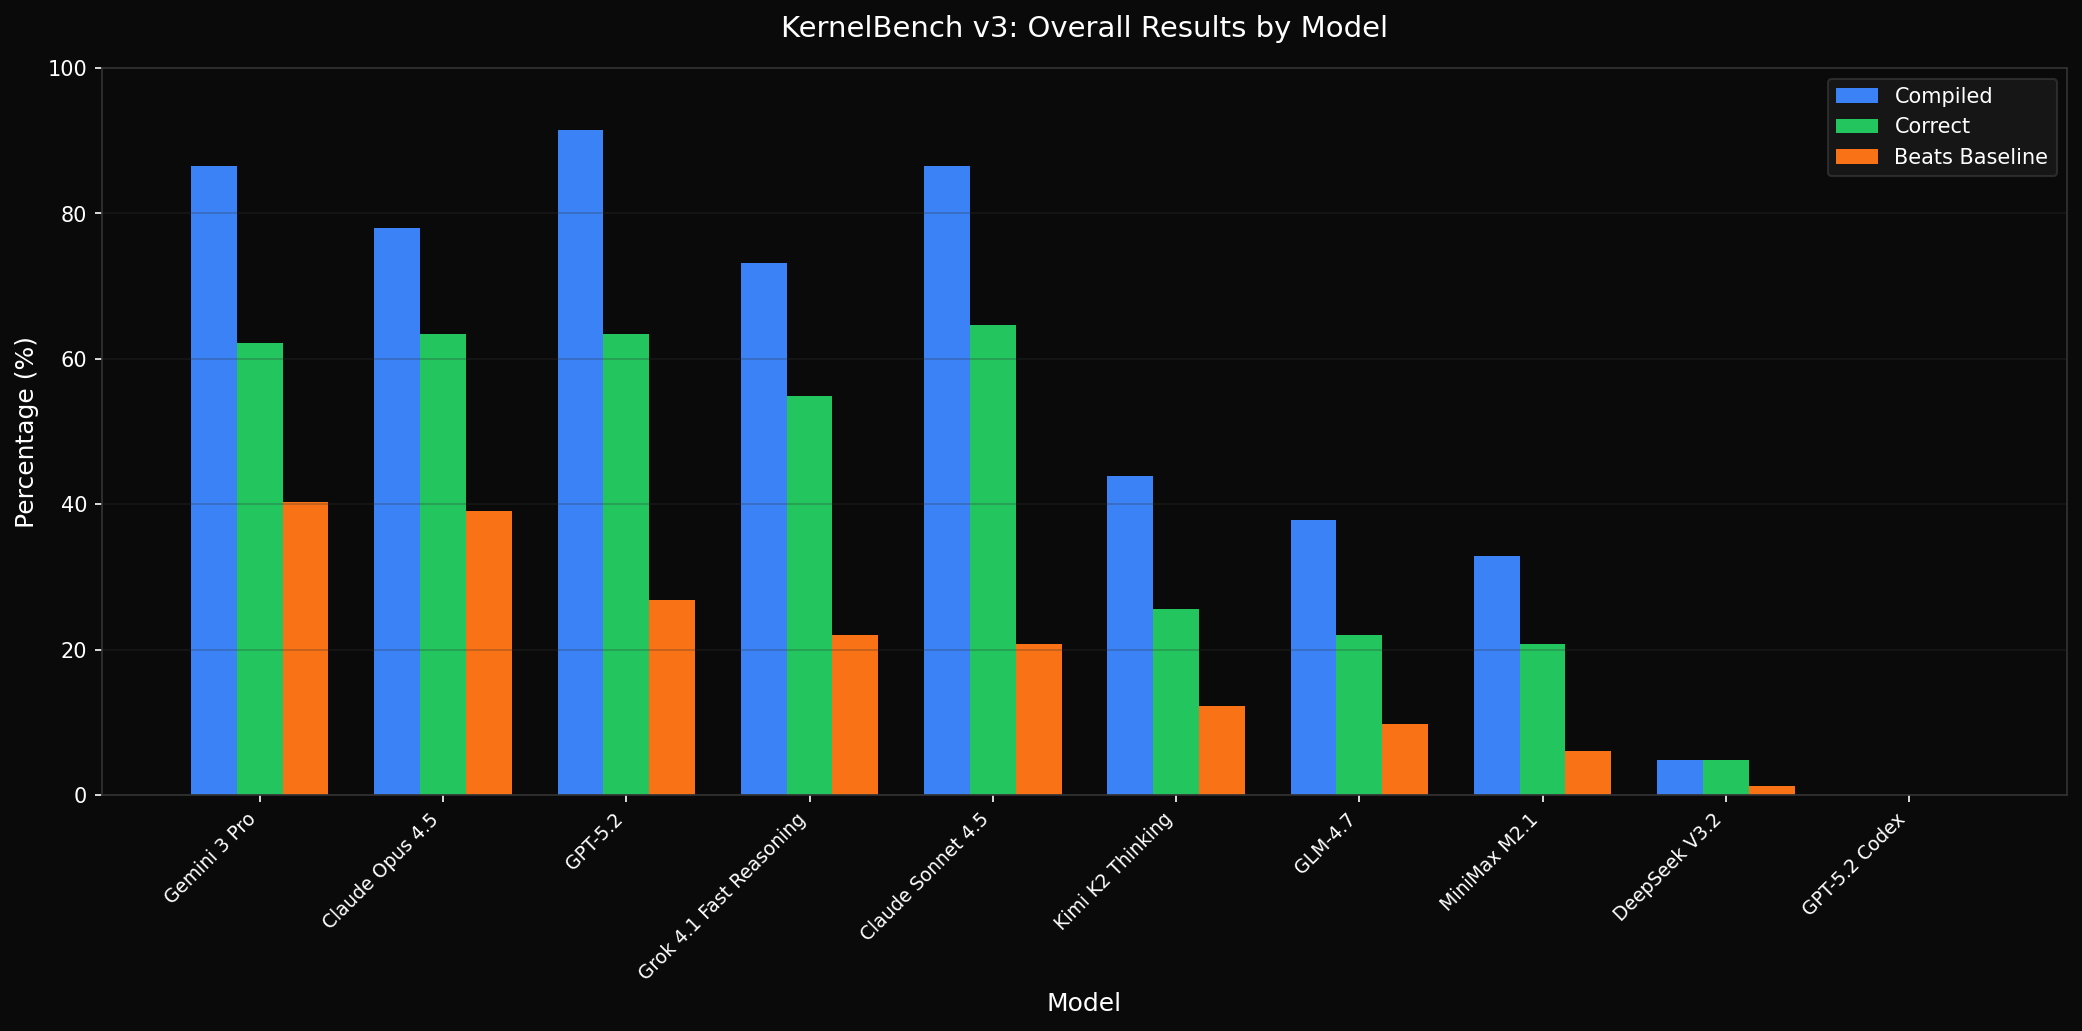
\includegraphics[width=0.95\linewidth]{figures/results_overall.png}
\caption{Overall results by model. Bars show the fraction of runs that compiled, were correct, and beat the baseline.}
\label{fig:overall}
\end{figure}

\noindent Figure~\ref{fig:overall} is sourced from the public dashboard export. GPT-5.2 Codex appears at 0\% there because the evaluation failed due to an API format mismatch in the OpenAI Codex endpoint, not model performance. We exclude GPT-5.2 Codex from the tables and aggregate statistics.

\begin{figure}[t]
\centering
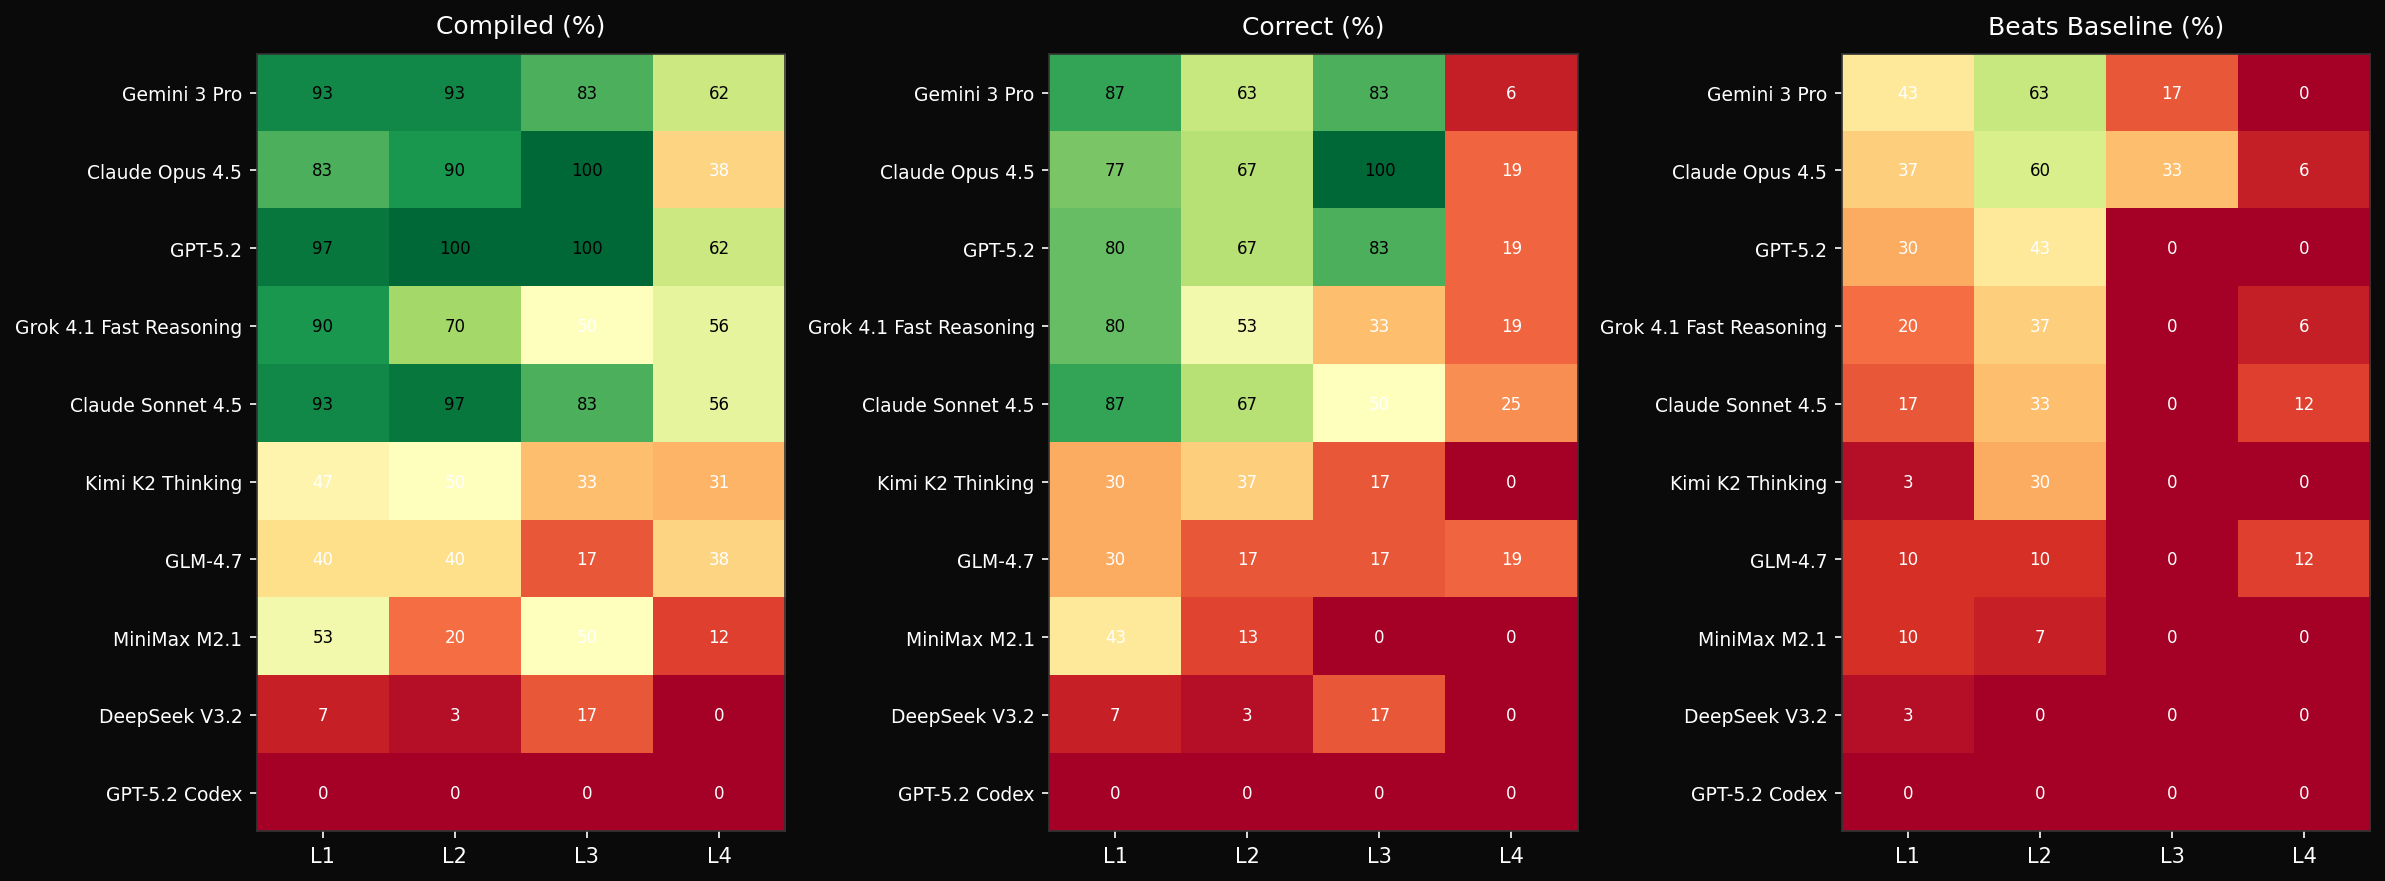
\includegraphics[width=0.98\linewidth]{figures/results_heatmap.png}
\caption{Heatmap of correctness and baseline-beating rates by level.}
\label{fig:heatmap}
\end{figure}

Table~\ref{tab:model-results} summarizes performance by model. Gemini 3 Pro and Claude Opus 4.5 produce the most baseline-beating kernels. GPT-5.2 has strong correctness but fewer baseline wins, indicating that correctness alone does not guarantee competitive performance.

The figures are sourced from the public dashboard export. GPT-5.2 Codex appears at 0\% there because the evaluation failed due to an API format mismatch in the OpenAI Codex endpoint, not model performance. We exclude GPT-5.2 Codex from the tables and aggregate statistics.

\begin{table}[t]
\centering
\caption{Model-level results across all problems and GPUs.}
\label{tab:model-results}
% Auto-generated from results.csv
\begin{tabular}{lrrrr}
\toprule
Model & Correct (\%) & Beat baseline (\%) & Beat baseline (n) & Total \\
\midrule
Gemini 3 Pro & 62.2 & 40.2 & 33 & 82 \\
Claude Opus 4.5 & 63.4 & 39.0 & 32 & 82 \\
GPT-5.2 & 63.4 & 26.8 & 22 & 82 \\
Grok 4.1 Fast Reasoning & 54.9 & 22.0 & 18 & 82 \\
Claude Sonnet 4.5 & 64.6 & 20.7 & 17 & 82 \\
Kimi K2 Thinking & 25.6 & 12.2 & 10 & 82 \\
GLM-4.7 & 22.0 & 9.8 & 8 & 82 \\
MiniMax M2.1 & 20.7 & 6.1 & 5 & 82 \\
DeepSeek V3.2 & 4.9 & 1.2 & 1 & 82 \\
\bottomrule
\end{tabular}

\end{table}

Table~\ref{tab:level-results} breaks down performance by difficulty level. Pass rates decline sharply at Level 4: only \PassRateLFour\% of runs pass correctness and \BeatRateLFour\% beat the baseline. These tasks include modern attention variants and quantized matmuls, and some use already-optimized Triton baselines.

\begin{table}[t]
\centering
\caption{Results by difficulty level.}
\label{tab:level-results}
% Auto-generated from results.csv
\begin{tabular}{crrrr}
\toprule
Level & Pass rate (\%) & Beat baseline (\%) & Beat baseline (n) & Total \\
\midrule
L1 & 57.8 & 19.3 & 52 & 270 \\
L2 & 43.0 & 31.5 & 85 & 270 \\
L3 & 44.4 & 5.6 & 3 & 54 \\
L4 & 11.8 & 4.2 & 6 & 144 \\
\bottomrule
\end{tabular}

\end{table}


\section{Discussion}
KernelBench v3 results reinforce two observations. First, baseline-beating kernels are rare even for top models. This aligns with METR's finding that kernel benchmarks can overstate capability when task design is weak~\cite{metr2025}. Second, performance collapses on Level 4 tasks, which emphasize modern attention and quantization patterns~\cite{fp8-formats,int4-quant}. These tasks are not just harder because of novelty but also because some baselines are already optimized Triton implementations~\cite{triton}, shrinking the remaining optimization headroom.

We also observe that correctness is not the limiting factor for all models. Several models achieve respectable correctness rates but lower baseline-beating rates, suggesting that the remaining gap is performance engineering rather than syntax or functional accuracy. For practical kernel engineering, models must reason about memory layout, kernel fusion, and hardware-specific bottlenecks.

Finally, cost remains a key practical constraint. The benchmark logs per-run token counts and estimated costs, enabling analysis of accuracy and speedup as a function of spend. This makes KernelBench v3 useful for evaluating cost-performance tradeoffs, not just raw capability.


\section{Limitations and Future Work}
KernelBench v3 is limited to single-GPU kernels and does not yet cover multi-GPU collective patterns. Correctness is evaluated on a single input per run with a fixed tolerance, which may miss some numerical edge cases. The benchmark also uses a fixed number of turns per task; some models might achieve better performance with longer optimization loops.

Future work includes adding multi-GPU tasks, expanding the Level 4 suite as new architectures emerge, and strengthening correctness checks with multi-seed or distributional testing. An open question is how to design evaluation protocols that reward robust kernel engineering without encouraging benchmark-specific shortcuts.


\section{Conclusion}
KernelBench v3 offers a focused, modern benchmark for evaluating whether LLMs can produce optimized GPU kernels. Across \TotalEvals{} runs, only \OverallBeatRate\% of evaluations beat the baseline, and Level 4 performance remains low. These results suggest that current models are helpful assistants for kernel development but are not yet autonomous kernel engineers. The benchmark and results are released to support ongoing research into reliable, performant code generation~\cite{kernelbench-v3-repo}.


\section*{Acknowledgements}
Thanks to the open-source kernel and inference community for their feedback and tooling. Special thanks to the KernelBench and METR teams for publicly documenting pitfalls and evaluation methodology.

\bibliography{kernelbench_v3}
\bibliographystyle{arxiv}

\newpage
\appendix

\section{Problem Lists}
\subsection{Level 1: Simple Operators}
\begin{table}[H]
\centering
\small
% Auto-generated from README.md
\begin{tabular}{ll}
\toprule
Problem & Description \\
\midrule
1\_Square\_matrix\_multiplication\_.py & Square matrix multiplication \\
2\_Standard\_matrix\_multiplication\_.py & Standard matrix multiplication \\
3\_Batched\_matrix\_multiplication.py & Batched matrix multiplication \\
4\_Matrix\_vector\_multiplication\_.py & Matrix-vector multiplication \\
8\_Matmul\_with\_irregular\_shapes\_.py & Matmul with irregular shapes \\
9\_Tall\_skinny\_matrix\_multiplication\_.py & Tall-skinny matrix multiplication \\
23\_Softmax.py & Softmax activation \\
26\_GELU\_.py & GELU activation \\
36\_RMSNorm\_.py & RMSNorm \\
40\_LayerNorm.py & LayerNorm \\
42\_Max\_Pooling\_2D.py & Max pooling 2D \\
47\_Sum\_reduction\_over\_a\_dimension.py & Sum reduction \\
63\_conv\_standard\_2D\_\_square\_input\_\_square\_kernel.py & 2D convolution \\
82\_conv\_depthwise\_2D\_square\_input\_square\_kernel.py & Depthwise 2D convolution \\
95\_CrossEntropyLoss.py & Cross-entropy loss \\
\bottomrule
\end{tabular}

\end{table}

\subsection{Level 2: Fused Operations}
\begin{table}[H]
\centering
\small
% Auto-generated from README.md
\begin{tabular}{ll}
\toprule
Problem & Description \\
\midrule
6\_Conv3d\_Softmax\_MaxPool\_MaxPool.py & Conv3D with pooling chain \\
17\_Conv2d\_InstanceNorm\_Divide.py & Conv2D + InstanceNorm fusion \\
37\_Matmul\_Swish\_Sum\_GroupNorm.py & Matmul + Swish + GroupNorm \\
40\_Matmul\_Scaling\_ResidualAdd.py & Matmul + scaling + residual \\
46\_Conv2d\_Subtract\_Tanh\_Subtract\_AvgPool.py & Conv2D + activation chain \\
52\_Conv2d\_Activation\_BatchNorm.py & Conv2D + BatchNorm fusion \\
55\_Matmul\_MaxPool\_Sum\_Scale.py & Matmul + pooling chain \\
59\_Matmul\_Swish\_Scaling.py & Matmul + Swish + scaling \\
66\_Matmul\_Dropout\_Mean\_Softmax.py & Matmul + dropout + softmax \\
73\_Conv2d\_BatchNorm\_Scaling.py & Conv2D + BatchNorm + scaling \\
82\_Conv2d\_Tanh\_Scaling\_BiasAdd\_Max.py & Conv2D + activation chain \\
85\_Conv2d\_GroupNorm\_Scale\_MaxPool\_Clamp.py & Conv2D + GroupNorm fusion \\
86\_Matmul\_Divide\_GELU.py & Matmul + GELU fusion \\
98\_Matmul\_AvgPool\_GELU\_Scale\_Max.py & Matmul + pooling + GELU \\
99\_Matmul\_GELU\_Softmax.py & Matmul + GELU + softmax \\
\bottomrule
\end{tabular}

\end{table}

\subsection{Level 3: Single Blocks}
\begin{table}[H]
\centering
\small
% Auto-generated from README.md
\begin{tabular}{ll}
\toprule
Problem & Description \\
\midrule
31\_VisionAttention.py & Vision attention mechanism \\
43\_MinGPTCausalAttention.py & Causal attention (MinGPT style) \\
44\_MiniGPTBlock.py & Full transformer block \\
\bottomrule
\end{tabular}

\end{table}

\subsection{Level 4: Novel Layers}
\begin{table}[H]
\centering
\small
% Auto-generated from README.md
\begin{tabular}{ll}
\toprule
Problem & Description \\
\midrule
1\_DeepSeek\_MLA.py & Multi-head Latent Attention with LoRA KV compression \\
2\_DeepSeek\_MoE.py & MoE with grouped expert routing \\
3\_GroupedQueryAttention.py & GQA with KV head expansion (Llama 3 style) \\
4\_FP8\_Matmul.py & FP8 E4M3 quantized matmul with tensor cores \\
5\_MoE\_GatedGEMM.py & MoE with fused gated dual GEMM (SwiGLU FFN) \\
6\_INT4\_Quantized\_GEMM.py & INT4 weight-only quant with group-wise dequant fusion \\
7\_GatedDeltaNet.py & Gated delta rule linear attention (ICLR 2025) \\
8\_KimiDeltaAttention.py & Channel-wise gated delta attention \\
\bottomrule
\end{tabular}

\end{table}


\section{Supplementary Tables}
\subsection{Results by GPU}
\begin{table}[H]
\centering
% Auto-generated from results.csv
\begin{tabular}{lrrrr}
\toprule
GPU & Pass rate (\%) & Beat baseline (\%) & Beat baseline (n) & Total \\
\midrule
B200 & 41.2 & 19.0 & 70 & 369 \\
H100 & 43.6 & 20.6 & 76 & 369 \\
\bottomrule
\end{tabular}

\end{table}

\subsection{Token and Cost Accounting}
\begin{table}[H]
\centering
% Auto-generated from results.csv
\begin{tabular}{lrr}
\toprule
Model & Total tokens & Estimated cost (USD) \\
\midrule
Claude Opus 4.5 & 4776623 & 35.13 \\
GPT-5.2 & 2111940 & 27.55 \\
Grok 4.1 Fast Reasoning & 6248298 & 21.89 \\
Claude Sonnet 4.5 & 2821243 & 12.57 \\
Gemini 3 Pro & 5372941 & 7.77 \\
MiniMax M2.1 & 5983144 & 4.04 \\
GLM-4.7 & 4192667 & 2.87 \\
Kimi K2 Thinking & 3035630 & 2.08 \\
DeepSeek V3.2 & 1040464 & 0.29 \\
\bottomrule
\end{tabular}

\end{table}


\end{document}
